\documentclass{article}\usepackage[]{graphicx}\usepackage[]{color}
%% maxwidth is the original width if it is less than linewidth
%% otherwise use linewidth (to make sure the graphics do not exceed the margin)
\makeatletter
\def\maxwidth{ %
  \ifdim\Gin@nat@width>\linewidth
    \linewidth
  \else
    \Gin@nat@width
  \fi
}
\makeatother

\usepackage{Sweavel}


\usepackage{verbatim,color,amssymb,epsfig}
\usepackage[usenames,dvipsnames]{xcolor}
\usepackage{fancyhdr}
\usepackage[letterpaper]{geometry}
\usepackage{pdfpages}
\usepackage[T1]{fontenc}
\usepackage[authoryear, sort]{natbib}
\usepackage{amsmath}
\usepackage{amssymb}
\usepackage[labelfont=bf]{caption}
\usepackage{floatrow}
\usepackage{setspace}
\usepackage{cleveref}

\setstretch{1.5}
\floatsetup[table]{style=Plaintop,footskip=2pt,captionskip=5pt}
\floatsetup{font={stretch={1.1}}}
\captionsetup{footfont=small}

\def\bbeta{\mbox{\boldmath $\beta$}}
\def\pr{\hbox{pr}}
\def\E{{\mathbf E}}
\def\code#1{\texttt{#1}}
\def\pkg#1{\textbf{#1}}
\def\proglang#1{\texttt{#1}}


\begin{document}



\begin{titlepage}
\author{Alex Asher}
\title{Semiparametric Analysis of Polygenic Gene-Environment Interactions in Case-Control Studies with caseControlGE}
\date{June 2018}
\maketitle
\thispagestyle{empty}

%%%%%%%%%%%%%%%%%%%%%%%%%%%%%%%%%
%%%% Abstract %%%%%%%%%%%%%%%%%%%
%%%%%%%%%%%%%%%%%%%%%%%%%%%%%%%%%
\section*{Abstract}\label{sec:Abstract}
Gene-environment interactions can be efficiently estimated in case-control data by methods that assume gene-environment independence in the source population, but until recently such techniques required parametric modelling of the genetic variables.  The \pkg{caseControlGE} package implements the methods of \citeauthor{Stalder2017} (2017, \emph{Biometrika}, \textbf{104}, 801-812) and \citeauthor{Wang2018unpublished} (2018, unpublished), which exploit the assumption of gene-environment independence without placing any assumptions on the marginal distributions of the genetic or environmental variables.  These methods are ideally suited for analyzing complex polygenic data for which parametric distributional models are not feasible.  In addition to the two estimators, the package also supplies a function to simulate case-control data and several helper functions for use on model objects.  Use of this package is illustrated by simulating and analyzing data from a case-control study of breast cancer.

\end{titlepage}
\newpage

\section{Introduction}

\subsection{caseControlGE package}

The \pkg{caseControlGE} package \citep{Asher2018R} contains tools for the analysis of case-control data using \proglang{R} \citep{R2018}.  It implements the methods of \citet{Stalder2017} and \citet{Wang2018unpublished}, both of which fall under the class of semiparametric retrospective profile likelihood estimators.  These methods are the first available to exploit the assumption of gene-environment independence while treating the genetic component nonparametrically.  As such, they are well suited to replace logistic regression as the preferred method in situations where parametric distributional models are not feasible, such as in the analysis of complex polygenic data.

\pkg{caseControlGE} contains three main functions: \code{simulateCC}, \code{spmle}, and \code{spmleCombo}, as well as several helper functions.  \Cref{sec:simulateCC} of this paper introduces \code{simulateCC} in the context of simulating case-control data analogous to the data analyzed in \cite{Wang2018unpublished}.  \Cref{sec:spmle} introduces \code{spmle} as a tool to analyze the simulated data, and \cref{sec:spmleCombo} introduces \code{spmleCombo} to conduct a more efficient analysis of the simulated data.

\subsection{Background}

Case-control studies are retrospective observational studies in which the sample consists of a group of healthy subjects and a group of diseased subjects.  A crucial aspect of the case-control design is that the outcome, disease status, is known \emph{before} sampling.  The ability to deliberately oversample diseased subjects makes the case-control design cost effective, which is why it is widely popular in studies of gene-environment interactions.

Given the genetic and environmental covariates $G$ and $E$, we assume the risk of disease $D$ in the underlying population follows the model
\begin{equation}
  \pr(D=1 \mid G,X) = H\{\beta_0 + m(G,X,\bbeta)\}, \label{eq:logisticRisk}
\end{equation}
where $H(x)=\{ 1 + \exp(-x)\}^{-1}$ is the logistic distribution function and $m(G,X,\bbeta)$ is a function that describes the joint effect of $G$ and $X$ and is known up to the unspecified parameters of interest $\bbeta$.

Given the retrospective nature of case-control sampling, it is surprising that standard prospective logistic regression can be used to obtain unbiased estimates of $\bbeta$ \citep{PrenticePyke1979}.  Logistic regression requires no assumptions about the joint distribution of $G$ and $E$, but it suffers from low power when estimating $G * E$ interaction effects.  To gain efficiency, \citet{ChatterjeeCarroll2005} exploited the assumption of gene-environment independence in the source population to maximize the retrospective likelihood while profiling out the distribution of $E$.  Their method is available as the function \code{snp.logistic} in the \emph{Bioconductor} package \pkg{CGEN} \citep{CGEN2012}.

The method of \citeauthor{ChatterjeeCarroll2005}, and subsequent methods utilizing the same retrospective profile likelihood framework, require a parametric model for the distribution of $G$ given $E$.  This becomes difficult as the number and complexity of genetic variables in the model grows.  Capitalizing on advances in high-throughput genomics, genome-wide association studies have identified scores of SNPs associated with complex diseases such as cancers and diabetes.  Modern case-control studies of gene-environment interactions need efficient methodology that allows for a flexible and arbitrarily complex genetic component, such as multiple correlated SNPs and/or continuous polygenic risk scores.

The method of \citet{Stalder2017} extends the retrospective profile likelihood framework of \citeauthor{ChatterjeeCarroll2005}, dispensing with the need to model $G$ parametrically.  When the population disease rate $\pi_1$ is known, the retrospective profile loglikelihood can be estimated (up to an additive constant) using just the case-control sample and without modeling the distribution of $G$.  When $\pi_1$ is unknown but the disease is rare, estimates can be obtained using the \emph{rare disease approximation} that $\pi_1 \approx 0$, which typically introduces negligible bias \citep{Stalder2017}.

\citet{Wang2018unpublished} proposed an improvement to the method of \citet{Stalder2017} that increases the efficiency of the estimates with no additional assumptions.  This development relies on the observation that the method of \citeauthor{Stalder2017} removes dependence on the distribution of the genetic and environmental variables in two different fashions; by treating the genetic and environmental variables symmetrically \citeauthor{Wang2018unpublished} generate two sets of parameter estimates that are combined to generate a more efficient estimate.

\subsection{Implementation}

The semiparametric method of \citet{Stalder2017} is implemented as the function \code{spmle} in \pkg{caseControlGE}, detailed in \cref{sec:spmle}.  Estimating the semiparametric profile likelihood is a computationally intensive process, and significant effort was invested in speeding up calculations.  Estimation functions, including the analytic gradient and hessian, are written in C++ and compiled using \pkg{Rcpp} \citep{Eddelbuettel2013Rcpp}, providing a tremendous speedup over native \proglang{R} code.  Extensive benchmarking and code profiling was conducted, and estimation functions were written to apply matrix operations to contiguous blocks of memory whenever possible, reducing memory latency and allowing modern processors to exploit data level parallelism and perform the same operation on multiple data points simultaneously.

The estimated semiparametric likelihood is maximized using the quasi-Newton optimizer \pkg{ucminf} \citep{Nielsen2016ucminf} using starting values from logistic regression.  \code{ucminf} is particularly well suited for this application because it allows us to precondition the optimization with the analytic hessian, and it evaluates the gradient after each call to the objective function.  Calculating the gradient along with the likelihood adds negligible computational complexity, so we call a single C++ function to compute them both, then return them separately to \code{ucminf}.  This leads \code{ucminf} to converge in roughly half the time of the next-fastest optimizers (several of the various \proglang{R} implementations of the BFGS algorithm tie for second place).  The unmatched speed of \code{ucminf} means we are willing to tolerate its bugs, which include occasionally declaring convergence before actually converging.  To address this, \code{spmle} checks the gradient at the reported optimum and restarts the optimization if necessary (with different starting values).

Computational complexity of the asymptotic covariance estimation, which contains a sum of the form $\sum_{i=1}^{n} \: \sum_{j=1}^{n} \: \sum_{k=1}^{n} \partial {\cal L}_{ijk}(\Omega) / \partial \Omega$, was reduced from $O(n^3)$ to $O(n^2)$ by storing intermediate values in a three-dimensional array.  This increases speed at the cost of memory usage, which climbs from $O(n)$ to $O(n^2)$, setting a practical limit on sample size in the low tens of thousands for average personal computers.  This is sufficient to analyze all but the largest case-control studies; covariance estimates for larger studies should be computed using the bootstrap.

Asymptotic covariance estimates for the Symmetric Combination Estimator of \citeauthor{Wang2018unpublished} converge slowly and unreliable in practice, often providing poor coverage.  \citeauthor{Wang2018unpublished} recommend a balanced bootstrap, with cases and controls resampled separately, to estimate covariance.  \pkg{caseControlGE} offers users with multicore computers the option to speed up computation by using multiple processors.  Parallelization is implemented using the \proglang{R} base package \pkg{parallel}, which is installed by default on all operating systems.  Parallelization on computers running Linux or macOS is done by forking the active \proglang{R} session, saving time and memory.  This option is unavailable in Windows, so parallelization is fractionally slower because a PSOCK cluster is created with a new instance of \proglang{R} running on each core.


\section{Simulating case-control data with simulateCC} \label{sec:simulateCC}

\subsection{Data description}

\cite{Wang2018unpublished} demonstrate the utility of their method by analyzing data from a case-control study of breast cancer.  This case-control sample is taken from a large prospective cohort at the National Cancer Institute: the Prostate, Lung, Colorectal and Ovarian (PLCO) cancer screening trial \citep{canzian2010comprehensive}.  The case-control study analyzed by \citeauthor{Wang2018unpublished} consists of 658 cases and 753 controls sampled from a cohort of 64,440 non-Hispanic, white women aged 55 to 74, of whom 3.72\% developed breast cancer \citep{pfeiffer2013risk}.  The data are available from the National Cancer Institute via a data transfer agreement, but cannot be distributed with the \pkg{caseControlGE} package.  Fortunately, we can use the \pkg{caseControlGE} function \code{simulateCC} to generate a similar data set for analysis.

Each of the 1411 subjects in the PLCO sample was genotyped for 21 SNPs that have been previously associated with breast cancer based on large genome-wide association studies.  These SNPs were weighted by their log-odds-ratio coefficients and summed to define a polygenic risk score (PRS).  A standardized version of this PRS, with mean zero and standard deviation one, was used as the genetic risk factor $G$ by \citeauthor{Wang2018unpublished}.  Early menarche is a known risk factor for breast cancer, and \citeauthor{Wang2018unpublished} used a binary indicator of whether the subject underwent early menarche as $E$ (age at menarche < 14).  Several environmental variables were recorded as part of the PLCO study, including body mass index (BMI).  There is some evidence that obese women have a reduced risk of breast cancer, so in our simulation we will consider BMI in addition to the variables modeled by \citeauthor{Wang2018unpublished}.

\subsection{Data simulation}

Genetic variables generated by \code{simulateCC} include SNPs and three distributions of continuous PRS: Normal(0,1), Gamma(shape=20, scale=20), and bimodal.  Environmental variables can be binary or Normal(0,1).  To simulate case-control data with \code{simulateCC}, we specify distributions for $G$ and $E$ and provide regression coefficients $\bbeta$ and intercept $\beta_0$ from \cref{eq:logisticRisk}.  The function \code{simulateCC} generates values of $G$ and $E$ for a simulated population, then simulates binary $D$ from its conditional distribution $(D \mid G, X, \beta_0, \bbeta)$.  A sample of $n_1$ cases and $n_0$ controls is taken from this simulated population.

To determine the appropriate distributions to use when simulating $G$ and $E$, we examine the PLCO data.  In doing so, it is important to keep in mind that the case control sample is not representative of the source population.  Case-control studies deliberately oversample cases, so the distribution of $G$ and $E$ in the sample may be quite different from the distribution of $G$ and $E$ in the population (especially for variables that are strongly correlated with disease status).  To accurately simulate the genetic and environmental variables from the PLCO study, we need to estimate their distributions \emph{in the source population}.

\citeauthor{Wang2018unpublished} report $\beta_G = 0.459$ with $p < 1e-4$, but they standardized $G$ to mean zero and standard deviation one \emph{in the case-control sample}.  $G$ has a strong positive effect on disease risk, indicating that the distribution of $(G|D=0)$ is meaningfully different from the distribution of $(G|D=1)$.  Specifically, $\mathbf{E}(G|D=1) > \mathbf{E}(G|D=0)$.  With a population disease rate of 0.0372, this implies $\mathbf{E_{\rm pop}}(G) \approx \mathbf{E}(G|D=0) < 0$, where the subscript pop emphasizes that the expectation is in the source population.

This causes no problem for \citeauthor{Wang2018unpublished}, but it presents us with the dilemma that $G \nsim \hbox{N}(0,1)$.  If we simulate $G \sim \hbox{N}(0,1)$ and use $\beta_G = 0.459$ as reported in \citeauthor{Wang2018unpublished}, our simulated $(D \mid G, X, \beta_0, \bbeta)$ will not match the distribution of the actual PLCO data.

If we did not have access to the PLCO data, our best option would be to approximate $\delta = \mathbf{E}(G|D=0)$, simulate $G \sim \hbox{N}(\delta, 1)$, and use $\bbeta$ as reported in \citeauthor{Wang2018unpublished}.  While we cannot distribute the PLCO data, we \emph{can} use it to estimate population parameters, so approximating $\delta$ is not necessary.  The simplest and most common way to estimate population parameters is to calculate them using just the controls.  Case-control designs are typically used to study relatively rare diseases, and the bias introduced by using the cases as a stand-in for the population is usually quite small.

When $\pi_1$ is known, it is possible to calculate unbiased estimates by weighting the cases and controls by $\pi_1$ and $(1 - \pi_1)$, respectively.  (This technique is employed to great effect by \citeauthor{Stalder2017}, and is the reason that \code{spmle} requires the user to specify a value for \code{pi1}.)

We return to the PLCO data to conduct an analysis similar to that of \citeauthor{Wang2018unpublished}, but with two environmental variables: the indicator of early menarche and BMI.  We will standardize the two continuous variables due to their very different scales, but to make our lives easier when we conduct subsequent simulations, we standardize them to have mean zero and standard deviation one \emph{in the source population}.

We calculate $\mathbf{\widehat{E}_{\rm pop}}(\rm PRS)$, $\mathbf{\widehat{E}_{\rm pop}}(\text{early menarche})$, and $\mathbf{\widehat{E}_{\rm pop}}(\rm BMI)$ by weighting the means within cases and controls by $\pi_1$ and $(1 - \pi_1)$, respectively.  We calculate $\widehat{\hbox{sd}}_{\rm pop}(\rm PRS)$ and $\widehat{\hbox{sd}}_{\rm pop}(\rm BMI)$ using the sample standard deviations among the controls only.  We have
\begin{align*}
  G = \frac{{\rm PRS} - \mathbf{\widehat{E}_{\rm pop}}(\rm PRS)}{\widehat{\hbox{sd}}_{\rm pop}(\rm PRS)}, && E_1 = \mathbf{I}(\texttt{age at menarche} < 14), && E_2 = \frac{{\rm BMI} - \mathbf{\widehat{E}_{\rm pop}}(\rm BMI)}{\widehat{\hbox{sd}}_{\rm pop}(\rm BMI)}.
\end{align*}
After this scaling, the distributions of $G$ and $E_2$ in the source population can be well approximated by uncorrelated $\hbox{N}(0, 1)$ random variables.  Binary environmental variable $E_1$ is also uncorrelated with $G$, and has a frequency of 0.745 in the population.  We fit a model in these variables to the PLCO data using \code{spmleCombo}, yielding the rest of the information we need to simulate case control data:
\begin{align*}
  \pi_1   & =    0.0372        & n_0          & =    753               & n_1          & =     658          \\
  G       & \sim \hbox{N}(0,1) & E_1          & \sim \hbox{Bin}(0.745) & E_2          & \sim \hbox{N}(0,1) \\
  \beta_G & =    0.450         & \beta_{E_1}  & =    0.143             & \beta_{E_2}  & =    -0.019        \\
          &                    & \beta_{GE_1} & =   -0.195             & \beta_{GE_2} & =    -0.040
\end{align*}
The logistic intercept $\beta_0$ is not consistently estimated by logistic regression or either of the semiparametric methods in \pkg{caseControlGE}, however it is typically of little interest.  The function \code{simulateCC} prints the population disease rate each time it runs, so we run \code{simulateCC} several times with different values of $\beta_0$.  Using a guess-and-check approach with increasing sample size as we get closer, we manipulate $\beta_0$ to match the disease rate observed in the source population.

\begin{Schunk}
\begin{Sinput}
#### Load the castControlGE package and set the random seed
library("caseControlGE")
set.seed(979)

#### Generate data with beta0 = -3 as a starting point
tmp = simulateCC(ncase=1000, ncontrol=1000, beta0 = -3, betaG_normPRS=0.450,
                 betaE_bin=0.143, betaE_norm=-0.019, betaGE_normPRS_bin=-0.195,
                 betaGE_normPRS_norm=-0.040, E_bin_freq=0.745)
\end{Sinput}
\begin{Soutput}

Disease prevalance: 0.0520909090909091 
\end{Soutput}
\begin{Sinput}
#### Disease rate too high, try beta0 = -4
tmp = simulateCC(ncase=1000, ncontrol=1000, beta0 = -4, betaG_normPRS=0.450,
                 betaE_bin=0.143, betaE_norm=-0.019, betaGE_normPRS_bin=-0.195,
                 betaGE_normPRS_norm=-0.040, E_bin_freq=0.745)
\end{Sinput}
\begin{Soutput}

Disease prevalance: 0.0212909427411371 
\end{Soutput}
\begin{Sinput}
#### Continue guessing, increasing sample size as we get closer (not run)
# tmp = simulateCC(ncase=1000, ncontrol=1000, beta0 = -3.5, betaG_normPRS=0.450, betaE_bin=0.143, betaE_norm=-0.019, betaGE_normPRS_bin=-0.195, betaGE_normPRS_norm=-0.040, E_bin_freq=0.745)
# tmp = simulateCC(ncase=10000, ncontrol=10000, beta0 = -3.4, betaG_normPRS=0.450, betaE_bin=0.143, betaE_norm=-0.019, betaGE_normPRS_bin=-0.195, betaGE_normPRS_norm=-0.040, E_bin_freq=0.745)
# tmp = simulateCC(ncase=100000, ncontrol=100000, beta0 = -3.4, betaG_normPRS=0.450, betaE_bin=0.143, betaE_norm=-0.019, betaGE_normPRS_bin=-0.195, betaGE_normPRS_norm=-0.040, E_bin_freq=0.745)
# tmp = simulateCC(ncase=100000, ncontrol=100000, beta0 = -3.41, betaG_normPRS=0.450, betaE_bin=0.143, betaE_norm=-0.019, betaGE_normPRS_bin=-0.195, betaGE_normPRS_norm=-0.040, E_bin_freq=0.745)
rm(tmp)
\end{Sinput}
\end{Schunk}

After several iterations (commented out for speed), we determined that \code{beta0 = -3.41} produces a population disease rate of 0.0372.  Now we generate our simulated PLCO data.
\begin{Schunk}
\begin{Sinput}
#### Set the random seed for reproducability
set.seed(70)

#### Generate a synthetic data set that has similar properties to the PLCO data
dat = simulateCC(ncase=658, ncontrol=753, beta0 = -3.41, betaG_normPRS=0.450,
                 betaE_bin=0.143, betaE_norm=-0.019, betaGE_normPRS_bin=-0.195,
                 betaGE_normPRS_norm=-0.040, E_bin_freq=0.745)
\end{Sinput}
\begin{Soutput}

Disease prevalance: 0.0362381630253141 
\end{Soutput}
\end{Schunk}

\subsection{Confirming the G-E independence assumption}

The function \code{simulateCC} returns a list with elements \code{D}, \code{G}, and \code{E}, which are numeric vectors or matrices.  We combine them into a \code{data.frame} to print the first 6 rows.
\begin{Schunk}
\begin{Sinput}
#### Examine the simulated data
kable(list(head(as.data.frame(dat)), table(dat$D, dnn="D")), caption="Simulated PLCO data, rows 1:6")
\end{Sinput}
\begin{table}
\caption{\label{tab:unnamed-chunk-3}Simulated PLCO data, rows 1:6}

\centering
\begin{tabular}[t]{r|r|r|r}
\hline
D & G & E.1 & E.2\\
\hline
0 & 0.1336533 & 1 & 0.3866567\\
\hline
0 & 0.4328288 & 0 & 1.4536655\\
\hline
0 & 0.3389738 & 1 & -1.0088425\\
\hline
0 & -1.4542346 & 1 & 0.7076604\\
\hline
0 & -1.0777144 & 1 & -0.2864078\\
\hline
0 & 1.4280646 & 1 & 1.6047819\\
\hline
\end{tabular}
\centering
\begin{tabular}[t]{l|r}
\hline
D & Freq\\
\hline
0 & 753\\
\hline
1 & 658\\
\hline
\end{tabular}
\end{table}

\end{Schunk}

Case-control data generated by \code{simulateCC} is sorted by disease status (which is why the first 6 rows do not have a single case), but the sample size is correct.  Before we calculate the \code{spmle}, we will check the assumption of gene-environment independence in the source population.  In our case, this check is largely perfunctory because we did not provide the arguments \code{regress\_E\_bin\_on\_G\_normPRS} or \code{regress\_E\_norm\_on\_G\_normPRS} to \code{simulateCC}, so the genetic and environmental variates were drawn from independent distributions.

But when analyzing real data, it is crucial to verify this assumption.  Violations of the $G$-$E$ independence assumption can introduce bias in the estimates of interaction parameters between the specific genetic and environmental variables in violation of $G$-$E$ independence (the other parameters in the model appear unaffected in simulation studies by \citeauthor{Stalder2017}).

We do this by checking for dependence between \code{G} and \code{E} in the controls.  Environmental variable $E_1$ is binary, so we use a two sample \emph{t}-test of $G$ over the two levels of $E_1$.  To test for dependence between $G$ and $E_2$, we conduct a correlation test.
\begin{Schunk}
\begin{Sinput}
#### Save the indices of all controls in dat
controls = which(dat$D == 0)

#### t-test of G over the levels of E1
t.test(dat$G[controls] ~ dat$E[controls, 1])
\end{Sinput}
\begin{Soutput}

	Welch Two Sample t-test

data:  dat$G[controls] by dat$E[controls, 1]
t = -0.72912, df = 317.01, p-value = 0.4665
alternative hypothesis: true difference in means is not equal to 0
95 percent confidence interval:
 -0.2265577  0.1040422
sample estimates:
mean in group 0 mean in group 1 
    -0.11633867     -0.05508089 
\end{Soutput}
\begin{Sinput}
#### correlation test between G and E2
cor.test(dat$G[controls], dat$E[controls, 2])
\end{Sinput}
\begin{Soutput}

	Pearson's product-moment correlation

data:  dat$G[controls] and dat$E[controls, 2]
t = -0.81291, df = 751, p-value = 0.4165
alternative hypothesis: true correlation is not equal to 0
95 percent confidence interval:
 -0.10088258  0.04188409
sample estimates:
        cor 
-0.02965047 
\end{Soutput}
\end{Schunk}
Now that we are satisfied that the assumption of gene-environment independence has not been violated, we can exploit this assumption using the two semiparametric retrospective methods of \pkg{caseControlGE}.

\section{Analyzing case-control data with spmle} \label{sec:spmle}

The function \code{spmle} is the backbone of \pkg{caseControlGE}; it is called on its own to evaluate the SPMLE of \citeauthor{Stalder2017}, and it is the key component of the Symmetric Combination Estimator of \citeauthor{Wang2018unpublished}.  Calling \code{spmle} is slightly different from calling other estimation commands like \code{lm} or \code{glm} because we do not specify the model formula to \code{spmle}.  Instead we specify which variables are genetic and which are environmental, and \code{spmle} fits the formula: \code{D {\raise.17ex\hbox{$\scriptstyle\sim$}} G * E}.

We fit the gene-environment interaction model with \code{spmle}, and compare it to the estimates from standard logistic regression.  We do not need to fit the logistic regression model with a call to \code{glm} because \code{spmle} fits a logistic regression model to obtain starting values.  This logistic regression model is returned with the fitted \code{spmle} object.
\begin{Schunk}
\begin{Sinput}
#### Fit the spmle to the simulated PLCO data
spmleFit1 = spmle(D=D, G=G, E=E, pi1=0.0372, data=dat)

#### Print coefficient estimates from spmle and the logistic model returned by spmle
kable(summary(spmleFit1)$coefficients, digits=4, caption="spmle, known pi1")
\end{Sinput}
\begin{table}

\caption{\label{tab:unnamed-chunk-5}spmle, known pi1}
\centering
\begin{tabular}[t]{l|r|r|r|r}
\hline
  & Estimate & Std. Error & z value & Pr(>|z|)\\
\hline
(Intercept) & -0.3226 & 0.1049 & -3.0755 & 0.0021\\
\hline
G & 0.5808 & 0.1033 & 5.6203 & 0.0000\\
\hline
E1 & 0.1762 & 0.1332 & 1.3225 & 0.1860\\
\hline
E2 & 0.0430 & 0.0565 & 0.7604 & 0.4470\\
\hline
G:E1 & -0.2426 & 0.1064 & -2.2807 & 0.0226\\
\hline
G:E2 & -0.0436 & 0.0432 & -1.0091 & 0.3129\\
\hline
\end{tabular}
\end{table}

\begin{Sinput}
kable(summary(spmleFit1$glm_fit)$coefficients, digits=4, caption="Logistic regression")
\end{Sinput}
\begin{table}

\caption{\label{tab:unnamed-chunk-5}Logistic regression}
\centering
\begin{tabular}[t]{l|r|r|r|r}
\hline
  & Estimate & Std. Error & z value & Pr(>|z|)\\
\hline
(Intercept) & -0.3014 & 0.1152 & -2.6160 & 0.0089\\
\hline
G & 0.5513 & 0.1111 & 4.9610 & 0.0000\\
\hline
E1 & 0.1549 & 0.1311 & 1.1814 & 0.2375\\
\hline
E2 & 0.0435 & 0.0562 & 0.7730 & 0.4395\\
\hline
G:E1 & -0.2263 & 0.1279 & -1.7695 & 0.0768\\
\hline
G:E2 & -0.0130 & 0.0574 & -0.2258 & 0.8213\\
\hline
\end{tabular}
\end{table}

\end{Schunk}
The parameter estimates are extremely similar between the two models, but the \code{spmle} has smaller standard errors for the interaction terms.  Logistic regression uncovers some evidence of a \code{G:E1} interaction between the PRS and early menarche, but the result is not significant at the 0.05 level.  The \code{spmle} is able to provide stronger evidence of a \code{G:E1} interaction because the estimated standard error of the \code{G:E1} coefficient is 20\% larger with logistic regression than the \code{spmle}, giving a variance increase of almost 45\%.

In this instance we know the true population disease rate $\pi_1=0.0372$.  If $\pi_1$ were unknown we would calculate the \code{spmle} under the assumption that $\pi_1 \approx 0$.  Calculating the rare disease approximation using \code{spmle} is as simple as specifying \code{pi1 = 0} in the function call.
\begin{Schunk}
\begin{Sinput}
kable(summary(spmle(D=D, G=G, E=E, pi1=0, data=dat))$coef, dig=4, cap="spmle, rare disease")
\end{Sinput}
\begin{table}

\caption{\label{tab:unnamed-chunk-6}spmle, rare disease}
\centering
\begin{tabular}[t]{l|r|r|r|r}
\hline
  & Estimate & Std. Error & z value & Pr(>|z|)\\
\hline
(Intercept) & -0.3253 & 0.1054 & -3.0857 & 0.0020\\
\hline
G & 0.5862 & 0.1054 & 5.5617 & 0.0000\\
\hline
E1 & 0.1791 & 0.1336 & 1.3404 & 0.1801\\
\hline
E2 & 0.0428 & 0.0566 & 0.7562 & 0.4495\\
\hline
G:E1 & -0.2436 & 0.1051 & -2.3175 & 0.0205\\
\hline
G:E2 & -0.0437 & 0.0416 & -1.0492 & 0.2941\\
\hline
\end{tabular}
\end{table}

\end{Schunk}
The estimates and standard errors are nearly identical to the model with known $\pi_1$, indicating that a valid estimator can be obtained even when the disease rate is unknown.

The function \code{spmle} returns an \code{S3} object of class \code{"spmle"}.  \pkg{caseControlGE} contains \code{spmle} methods for all applicable \code{S3} generics, such as \code{summary.spmle}, \code{print.spmle}, \code{confint.spmle}, etc.  If the function \code{anova} is called on \code{spmle} objects, the method \code{anova.spmle} is used to calculate likelihood ratio tests of the models.  This is a valid way to test full vs reduced \code{spmle} models because the loglikelihood reported by \code{logLik.spmle} is accurate up to an additive constant. However, \code{anova} should not be used to compare an \code{spmle} object to a model fit by a different method.

Body mass index does not appear to be a significant predictor in this model.  The coefficients for the $E_2$ main effect and the $G*E_2$ interaction are near zero and both terms have large $p$ values, so we fit a reduced model without BMI.  To demonstrate the options controling optimization, we disable hessian preconditioning and supply bad starting values to the optimizer.
\begin{Schunk}
\begin{Sinput}
#### Fit the reduced spmle with bad starting values
spmleRed = spmle(D=D, G=G, E=E[,1], pi1=0.0372, data=dat, startvals=rep(NA, 4),
                 control=list(use_hess=FALSE))
\end{Sinput}
\begin{Soutput}
ucminf retry 1 of 2 
\end{Soutput}
\begin{Sinput}
summary(spmleRed)
\end{Sinput}
\begin{Soutput}

Call:
spmle(D = D, G = G, E = E[, 1], pi1 = 0.0372, data = dat, control = list(use_hess = FALSE), 
    startvals = rep(NA, 4))

Pearson Residuals: 
    Min       1Q   Median       3Q      Max  
-1.9511  -0.9175  -0.6480   1.0055   2.1736  

Coefficients:
            Estimate Std. Error z value Pr(>|z|)    
(Intercept)  -0.3221     0.1048  -3.075  0.00211 ** 
G             0.5808     0.1034   5.616 1.96e-08 ***
E[, 1]        0.1737     0.1331   1.305  0.19187    
G:E[, 1]     -0.2400     0.1064  -2.256  0.02408 *  
---
Signif. codes:  0 '***' 0.001 '**' 0.01 '*' 0.05 '.' 0.1 ' ' 1

    Null deviance: 1949.7  on 1410  degrees of freedom
Residual deviance: 1848.1  on 1407  degrees of freedom
AIC: 1856.1 
UCMINF retries: 1, iterations: 14, max gradient at convergence: 4.917e-08
\end{Soutput}
\end{Schunk}


and compare it to the full model using \code{anova}


\section{Analyzing case-control data with spmleCombo} \label{sec:spmleCombo}

In the code below we coerce \code{dat} into a \code{data.frame} and drop $E_2$ from the \code{data} that is passed to \code{spmle}.
% spmleRed = spmle(D=D, G=G, E=E.1, pi1=0.0372, data=as.data.frame(dat)[,-4])





%%%%%%%%%%%%%%%%%%%%%%%%%%%%%%%%%
%%%% Bibliography %%%%%%%%%%%%%%%
%%%%%%%%%%%%%%%%%%%%%%%%%%%%%%%%%
\bibliographystyle{biomAbhra}
\bibliography{RJCrefs_05-30-2018}

% 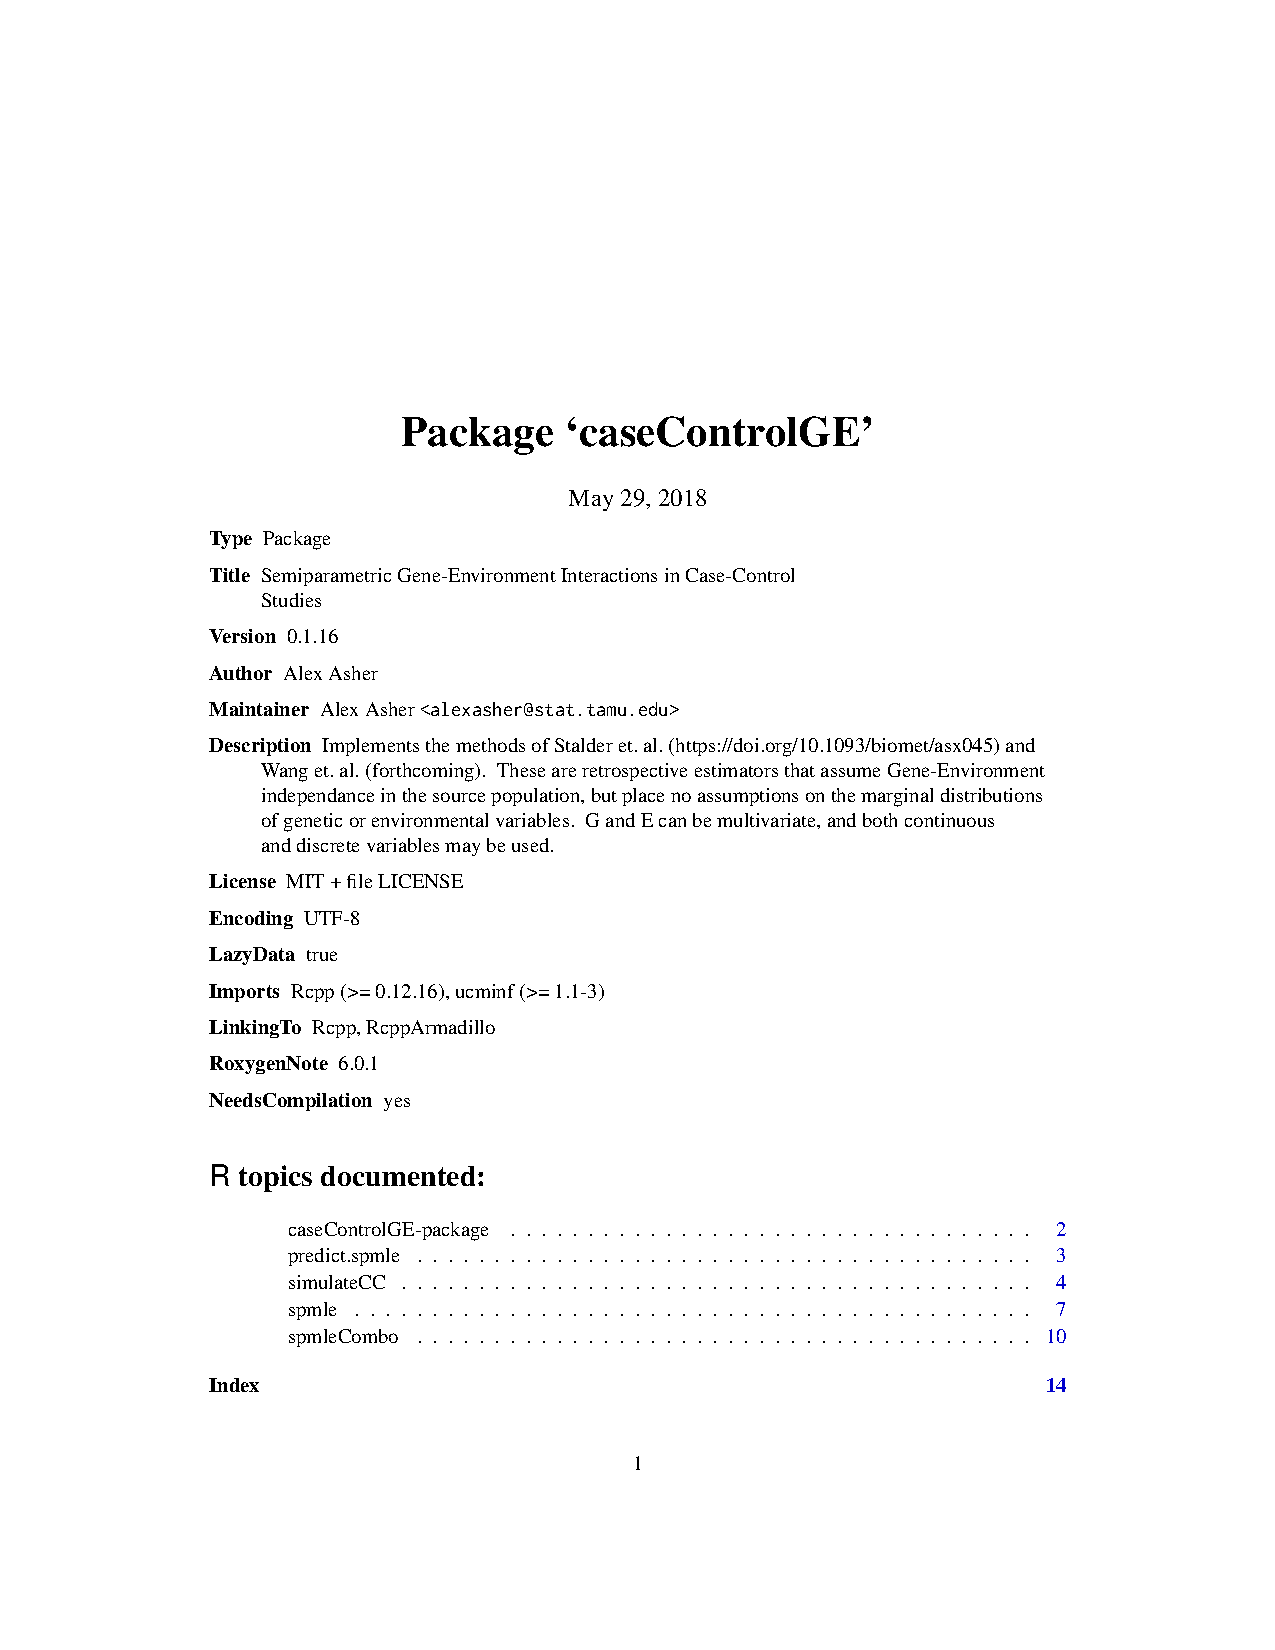
\includepdf[pages=-, fitpaper=true]{/home/alex/Research/Tianying/caseControlGE/caseControlGE}

\end{document}
